\section{Introduction}

%%% KM: Need to put in cross section for ZZ production.
%%%%%%%%%%%%%%%

The self-interaction of the gauge bosons ($W$, $Z$, and photon) 
is a consequence of the non-Abelian gauge symmetry of the Standard Model (SM). 
The gauge boson self-interactions appear as vertices involving three 
gauge bosons, and result in the production of pairs of bosons 
as shown in Figures~\ref{figure:diboson_feynman}-\ref{fig:wz_feynman}. 
This pair production of vector bosons is a very interesting process 
because it allows us to test how they couple to one another, something 
which one cannot do by producing them one at a time. 
The study of diboson production thus directly tests the predicted 
SM couplings. 

\par
Production of $W$ boson pairs involves both $WW\gamma$ and $WWZ$ couplings.
Production of $WZ$ involves the $WWZ$ triple gauge coupling (TGC).
Production of $ZZ$ involves $ZZ\gamma$ and $ZZZ$ couplings.
The study of $WZ$ production allows one to search for anomalous $WWZ$ coupling 
independent of the $WW\gamma$ coupling in contrast to $WW$ production.
Observations of anomalous couplings would be an indication of new physics.
Also, Higgs boson may decay into $WW$ or $ZZ$ pairs, giving rise to the same 
final state as the one that is studied in diboson production. 
In addition, Higgs itself can be produced together with one 
vector boson giving the same final state. 

\par
Diboson production was first seen at the Tevatron proton-antiproton 
collider~\cite{Hobbs:2010yg, CDF-diboson-lvjj-2010}, 
and then studied at LEP II where a  pair of $W$ bosons was created from 
electron-positron annihilation. 
Later still, $WZ$ production was seen at the Tevatron, and finally, more 
recently, $ZZ$ production has also been discovered~\cite{Hobbs:2010yg}.
%%%%%%%
\begin{figure}[h!] {\centering
    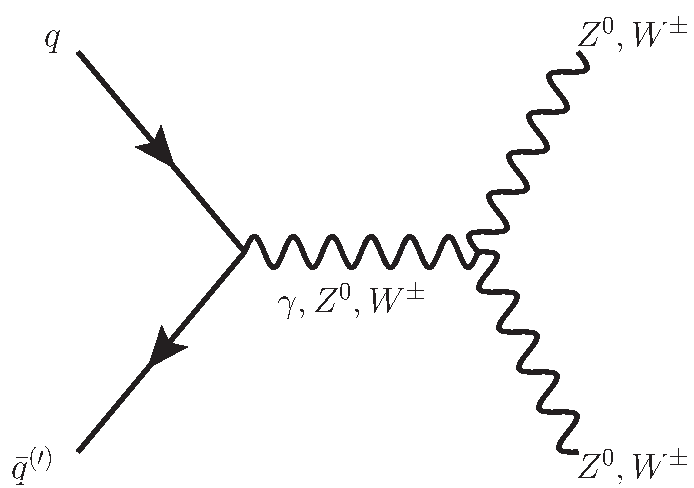
\includegraphics[width=0.4\textwidth]{figures/diboson_generic.pdf}
    \caption{Leading order diagram for $WW$ and $ZZ$ production via
  quark-antiquark annihilation involving the trilinear gauge coupling.}
    \label{figure:diboson_feynman}}
\end{figure}
%%%%%%%
%%%%%%%
\begin{figure}[h!] {\centering
\unitlength=0.33\linewidth
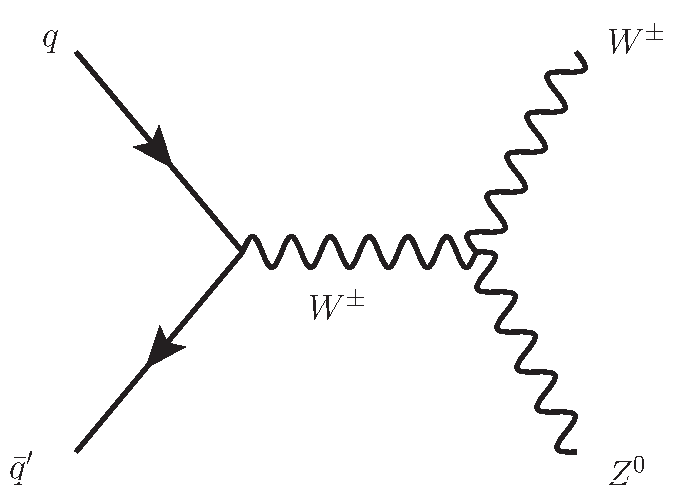
\includegraphics[width=0.33\textwidth]{figures/wz_schannel.pdf}
\put(-0.60,0.0){(a)} 
\unitlength=0.33\linewidth
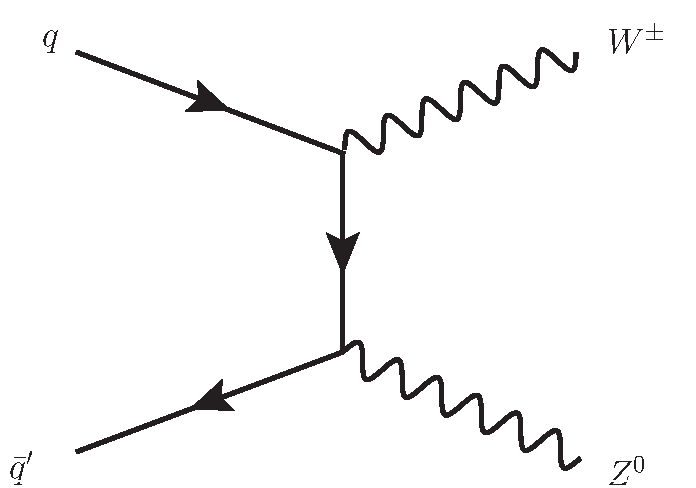
\includegraphics[width=0.33\textwidth]{figures/wz_tchannel.pdf}
\put(-0.60,0.0){(b)} 
\caption{Leading order (a) $s$-channel and (b) $t$-channel diagrams for
  $WZ$ production at the LHC. The $t$-channel diagram for $WW$ production 
  is also the same as (b) except that $Z$ is replaced by $W$ in the 
  outgoing leg.} 
\label{fig:wz_feynman}}
\end{figure}
%%%%%%%
%%%%%%%%%%%%%%%

This note describes two studies of diboson production -- $WW$, $WZ$, and 
$ZZ$ -- using data collected by the Compact Muon Solenoid (CMS) experiment~\cite{JINST} at $\sqrt{s}=7$~TeV. The first study uses an integrated luminosity of 1~fb${}^{-1}$ and considers events with a leptonically 
decaying $W$ or $Z$ boson  ($W\to\ell\nu$ or $Z\to\ell\ell$, where 
$\ell=e,\mu$) and one other $W$ or $Z$ boson that decays to $q\bar{q}$. The second study is that of $ZZ$ diboson production in the channel where one of the $Z$-boson decays to charged leptons ($Z\to\ell\ell$, with $\ell=e,\,\mu$) while the other decays to a pair of neutrinos ($Z\to\nu\nu$). A total integrated luminosity of 700~pb${}^{-1}$ is used by this second study.


The $W$ and $Z$ masses differ by about 10 GeV. However, the mass resolution 
of the CMS detector is insufficient to distinguish between the $W\to jj$ 
and $Z \to jj$ decay processes. 
Therefore, our signal contains an admixture of $WW$ and $WZ$ events in case 
of lepton + 2 jets + $\met$ final state.
Similarly, we have admixture of $ZZ$ and $WZ$ signal in case 
of 2 leptons + 2 jets final state.
  
The production cross section (at next-to-leading order (NLO) in perturbative 
QCD calculations) for $WW$ at LHC is 47 pb and for $WZ$ it is 18 pb. The NLO expectation for $ZZ$ is $5.1$~pb$^{-1}$ from MCFM.

\subsection{Why study diboson production in non-leptonic decay modes ?}
The advantage of reconstructing $WW$, $WZ$, and $ZZ$ in 
$\ell\nu jj$ or $\ell\ell jj$ decay modes over 
the purely leptonic channels is the larger branching fraction to jets, 
at the expense of larger backgrounds, mainly from $W/Z$+jets.
Compared to the pure $WW$ leptonic diboson decay the semi-leptonic 
process has the ability to  provide a direct handle on the boson transverse 
momentum. 
The sensitivity to very high boson $p_T$ makes this process particularly 
useful as a probe of the gauge structure (symmetries) at high energies 
where we anticipate new physics.
On the flip side, this channel is beset by a large background from 
single $W$ boson produced in association with quarks and/or gluons.

